\subsection{Visual Perception: Illusions and Gestalt Theory}
Visual perception is the process of extracting meaning from sensory information. It is concerned with recognition and understanding.
Vision is an easier process concerned with detecting color, shapes or edges of objects. Vision does not necessary require an understanding of the world surrounding us.\\
The Gestaltists, a group psychologists, identified a number of properties that can be regarded as innate to all humans. \\
Gestalt Laws: methods that the brain uses to simplify recognition by ordering them
\begin{enumerate}
\item Proximity: Objects that are close in space or time tend to be perceived together. This can be used e.g. for UI arrangement of buttons or information.
\item Common fate: Principle – Objects that ''move” together are seen as related
\item Prägnanz -- Law of Good Gestalt: Complex an unknown figures are automatically separated into known simple forms to make sense of them
\item Closure: Tendency to see things as complete objects even though there may be gaps in the shape of the objects. Closed figures are perceived more easily than incomplete or open figures.
\item Continuity: Tend to perceive smooth, continuous patterns instead of disjoint, interrupted patterns.
\item Similarity: Similar figures tend to be grouped together.
\item Part-whole relationships
\item Symmetry
\item Area Principle (also called the smallness principle): Objects with small area tend to be seen as the figure, not the ground.
\item Surroundedness Principle: An area that is surrounded will be seen as the figure and the area that surrounds will be seen as the ground.
\end{enumerate}
Other Principles of Perception:
\begin{itemize}
\item Stimulus Intensity: We respond first to the intensity of a stimulus and only then do we begin to process its meaning.
\item Proportion: can be used to represent logical hierarchies (e.g. font size of headings, subheadings...)
\item[$\rightarrow$] Golden Ratio: $\frac{a+b}{a}=\frac{a}{b}$The golden ratio expresses the relationship between two aspects of a form such as height to width and must equal 0.618; is seen as aesthetic
\item[$\rightarrow$] Fibonacci: A sequence of numbers in which each number is the sum of the two preceding numbers. The relationship between the numbers in the Fibonacci series is similar to the golden ratio.
\item Screen Complexity (Tullis, 1984): can be used to calculate the relative complexity, and therefore the difficulty, of a design. This measure of complexity uses information theory (Shannon \& Weaver, 1949) $C = -N \sum\limits_{n=1}^m p_n \log_2 p_n$ with 
\begin{itemize}
\item $C$ = complexity of the system in bits
\item $N$ = total number of events (widths or heights)
\item $m$ = number of event classes (number of unique widths or heights)
\item $p_n$ = probability of occurrence of the $n^{th}$ event class (based on the frequency of events within that class)
\end{itemize}
Calculating screen complexity:
\begin{enumerate}
\item Place a rectangle around every screen element
\item Count the number of elements and the number of columns (vertical alignment points)
\item Count the number of elements and the number of rows (horizontal alignment points) 
\item[$\rightarrow$] lowering these numbers reduces visual complexity (law of common fate, closure) 
\end{enumerate}
\begin{figure}[h!]
	\begin{subfigure}{.7\textwidth}
	\centering
	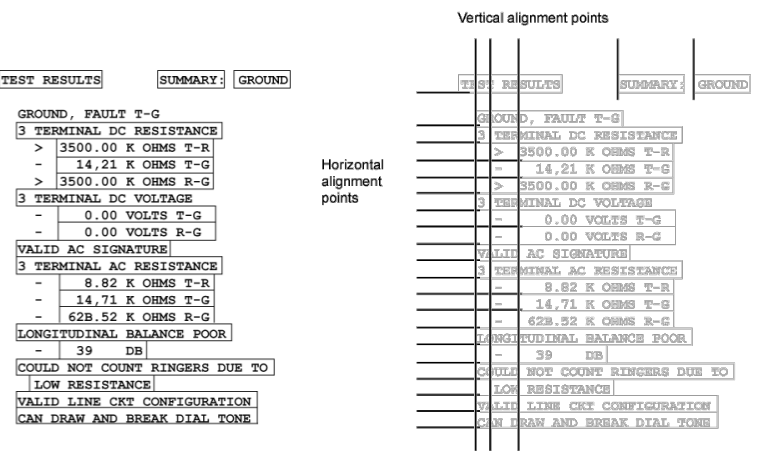
\includegraphics[width=.7\textwidth]{img/ch04_sc}
	\subcaption{Complexity Analysis}
	\end{subfigure}
	\begin{subfigure}{.5\textwidth}
	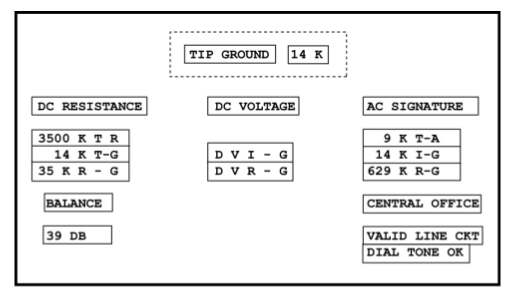
\includegraphics[width=.5\textwidth]{img/ch04_sc1}
	\centering \subcaption{Improved Interface}
	\end{subfigure}
	\caption{Example}
\end{figure}
\item[$\rightarrow$] Comber and Maltby (1997): both overly simple and overly complex screens low in usability (in terms of Effectiveness, Learnability, Attitude)
\end{itemize}
\textbf{Depth Perception}
Types of depth cues:\\
\begin{itemize}
\item Primary depth cues (relevant e.g. to immersive virtual reality systems)
\begin{itemize}
\item retinal disparity: As our eyes are approximately 7cm apart, each retina receives a slightly different image of the world. This is processed by the brain and interpreted as distance information.
\item Stereopsis: Process by which the different images of the world received by each eye are combined to produce a single three-dimensional experience.
\item Accommodation: A muscular process by which we change the shape of the lens in our eyes in order to create a sharply focused image. The information from the muscles is unconsciously used for depth information.
\item Convergence: Over distances of 2-7m we move our eyes more and more inwards to focus on an object at these distances. This process is used to provide additional depth information.
\end{itemize}
\item Secondary depth cues (more relevant e.g. to non-immersive applications such as games)
\begin{itemize}
\item Light and shade: An object with light and shadow improves the depth perception.
\item Linear perspective
\item Height in the horizontal plane
\item Motion parallax: Near objects are perceived to flash by quickly, objects further away as slower.
\item Overlap: e.g. overlapping windows in a GUI
\item Relative size: see sun + cloud
\item Texture gradient: textured surfaces appear closer
\end{itemize}
\end{itemize}
\subsection{Usability: Goals -- Principles -- Guidelines}
\begin{itemize}
\item Usability Goal -- Easy to use: most people do not want to struggle with tools are interested in completing their tasks
\item Design Principle -- Simplicity: Simple things require little effort and can often be accomplished without much thought. If interaction designs are guided by the principle of simplicity, they will be easier to use.
\item Project Guideline -- Dialog Boxes: All dialogue boxes should present only the basic functions that are most often used and that other, less used functions can be accessed using an expandable dialogue with a link for ''More Options”.
\end{itemize}
\subsection{Colors}
Additive (displays) and subtractive (printed) color mixing.\\
\textbf{Limitations}: 
\begin{itemize}
\item Blue Color is on the edge of the spectrum $\rightarrow$ Avoid using blue color for small and tiny elements.
\item The ability to distinguish color is directly related to the size of an object!
\item Shapes are identified by their edges. Edges are faster identified by lines than by colors.
\item Better color perception in the middle of the focus.
\item About 8\% of male (0.4\% of female) have deficiencies to perceive colors correctly. Most common deficiency is detection of green
\item Colors may cause problems leading to divided attention (as shown in Stroop test)
\item Colors may cause emotional response: varies depending on culture, age, sex $\rightarrow$ Industries, professional communities, corporate have their own colour connotations
\end{itemize}
\textbf{Colors for Design -- Color Coding -- Optimal Colors}
\begin{itemize}
\item For Clarification, Relation, Differentiation: e.g. Subway Maps
\item Support finding: e.g. important element in a text
\item Comprehension, Retention and Recall: e.g. Levels of danger, different measurements in a scatter plot etc.
\item Color coding can improve recall, search-and-locate tasks, decision judgements $\rightarrow$ overall performance but does not replace good structure!
\item Avoid any incompatible color combination, e.g. bright red on blue (background to foreground contrast)
\item Color presentation and perception change with medium and display technology; light in the workspace may influence color perception
\item Thorell \& Smith: red, blue, green and yellow are most beneficial in learning environments
\item Using a color code: Max 4 main colors, each having max 4 variants; structure the content and identify the content that should be supported with a color
\end{itemize}
\subsection{Hearing}
\textbf{Loudness} (dB): dB is a logarithmic scale; Frequency range of hearing 20Hz-20kHz\\
\textbf{Four Stages of Auditory Perception}
\begin{itemize}
\item Transduction: Translation of sound vibrations into neural impulses
\item Auditory grouping: Segregation into separate streams + Integration of sound in coherent streams (based on similar harmonic, frequency, location etc.)
\item Scene Analysis
\item Interpretation
\end{itemize}
\textbf{Audio User Interfaces}: Vision and Hearing go together, but audio can give impression from area that are beyond vision (audio can tell your eyes where to look). However, people become habituated to continuous sounds and ignore important sound based information. Continuous sounds requires resources from the human, even if it is a continuous sound, leading to additional stress. Audio can be perceived faster than visual cues. Audio is transitory! Vision is often not!\\
\textbf{(Non-)Speech}: We can speak faster than we can write, but spoken interaction contains more redundancy in terms of content. Speech requires knowledge of language. We can read faster than we can listen. It is often therefore more efficient to read than to listen. Listening is a liner task. Reading can jump! Auditory feedback can be non-speech. Beyond simple forms, sounds must be learned or familiar. They can be annoying and ambiguous and there are not so many expressions possible.\\
$\rightarrow$ Use of Sound:
\begin{itemize}
\item Redundant Coding: E.g. the ``click'' sound when pressing a GUI button\\
$\rightarrow$ redundant coding aids recalling an interaction by giving additional association\\
$\rightarrow$ can increase efficiency for tasks, as experts can react faster (on sound only)\\
$\rightarrow$ people with deficits (e.g. color blindness) may benefit from redundant coding\\
$\rightarrow$ Can be used for emotion (e.g. the ``miauw'' sound of my camera)\\
$\rightarrow$ Most important: Positive / Negative-Feedback
\item Speech applications
\end{itemize}
Use Case: Nomadic Radio	